
%402
\section{Sistemas de Ecuaciones Lineales Simultáneas}

\subsection{Sistemas de Dos Ecuaciones Lineales}

 Supongamos que $a_{i}, b_{i}, c_{i}, i=1,2$ son número dados:
	$$\begin{cases}
		a_{1}x+b_{1}y=c_{1}\\
		a_{2}x+b_{2}y=c_{2}\\
	\end{cases}
	$$
	En el sistema anterior, nuetro objetivos es encontrar dos números $x,y$ tales que cumplan ambas ecuaciones simultaneamente.



	\begin{problema}
		La soluci\'on del sistema 
		$$\begin{cases}
			x+y=7\\
			x-y=3
		\end{cases}
		$$ es $x=5,y=2.$
	\end{problema}
	



	A continuaci\'on, ejemplificaremos algunos de los m\'etodos más comunes para resolver sistemas de ecuaciones.

%

\[
	\label{spi151}
	2x-y=4
\]
\[	
	\label{spi152}
	x+2y=-3
\]		

	


{M\'etodo de sustituci\'on} 
	Despejando de \eqref{spi151}, obtenemos
	$$y=2x-4.$$
	
	Sutituyendo en \eqref{sp152}, obtenemos
	$$
	x+2(2x-4)=-3.
	$$
	


{M\'etodo de igualaci\'on}
	Despejando de \eqref{spi151}, obtenemos
	$$y=2x-4.$$
	
	Despejando de \eqref{sp152}, obtenemos
	$$y=-\dfrac{3+x}{2}.$$
	
	Igualando ambos lados derechos, obtenemos
	$$
	2x-4=-\dfrac{3+x}{2}.
	$$



{M\'etodo gráfico}
	\begin{figure}
		\centering
		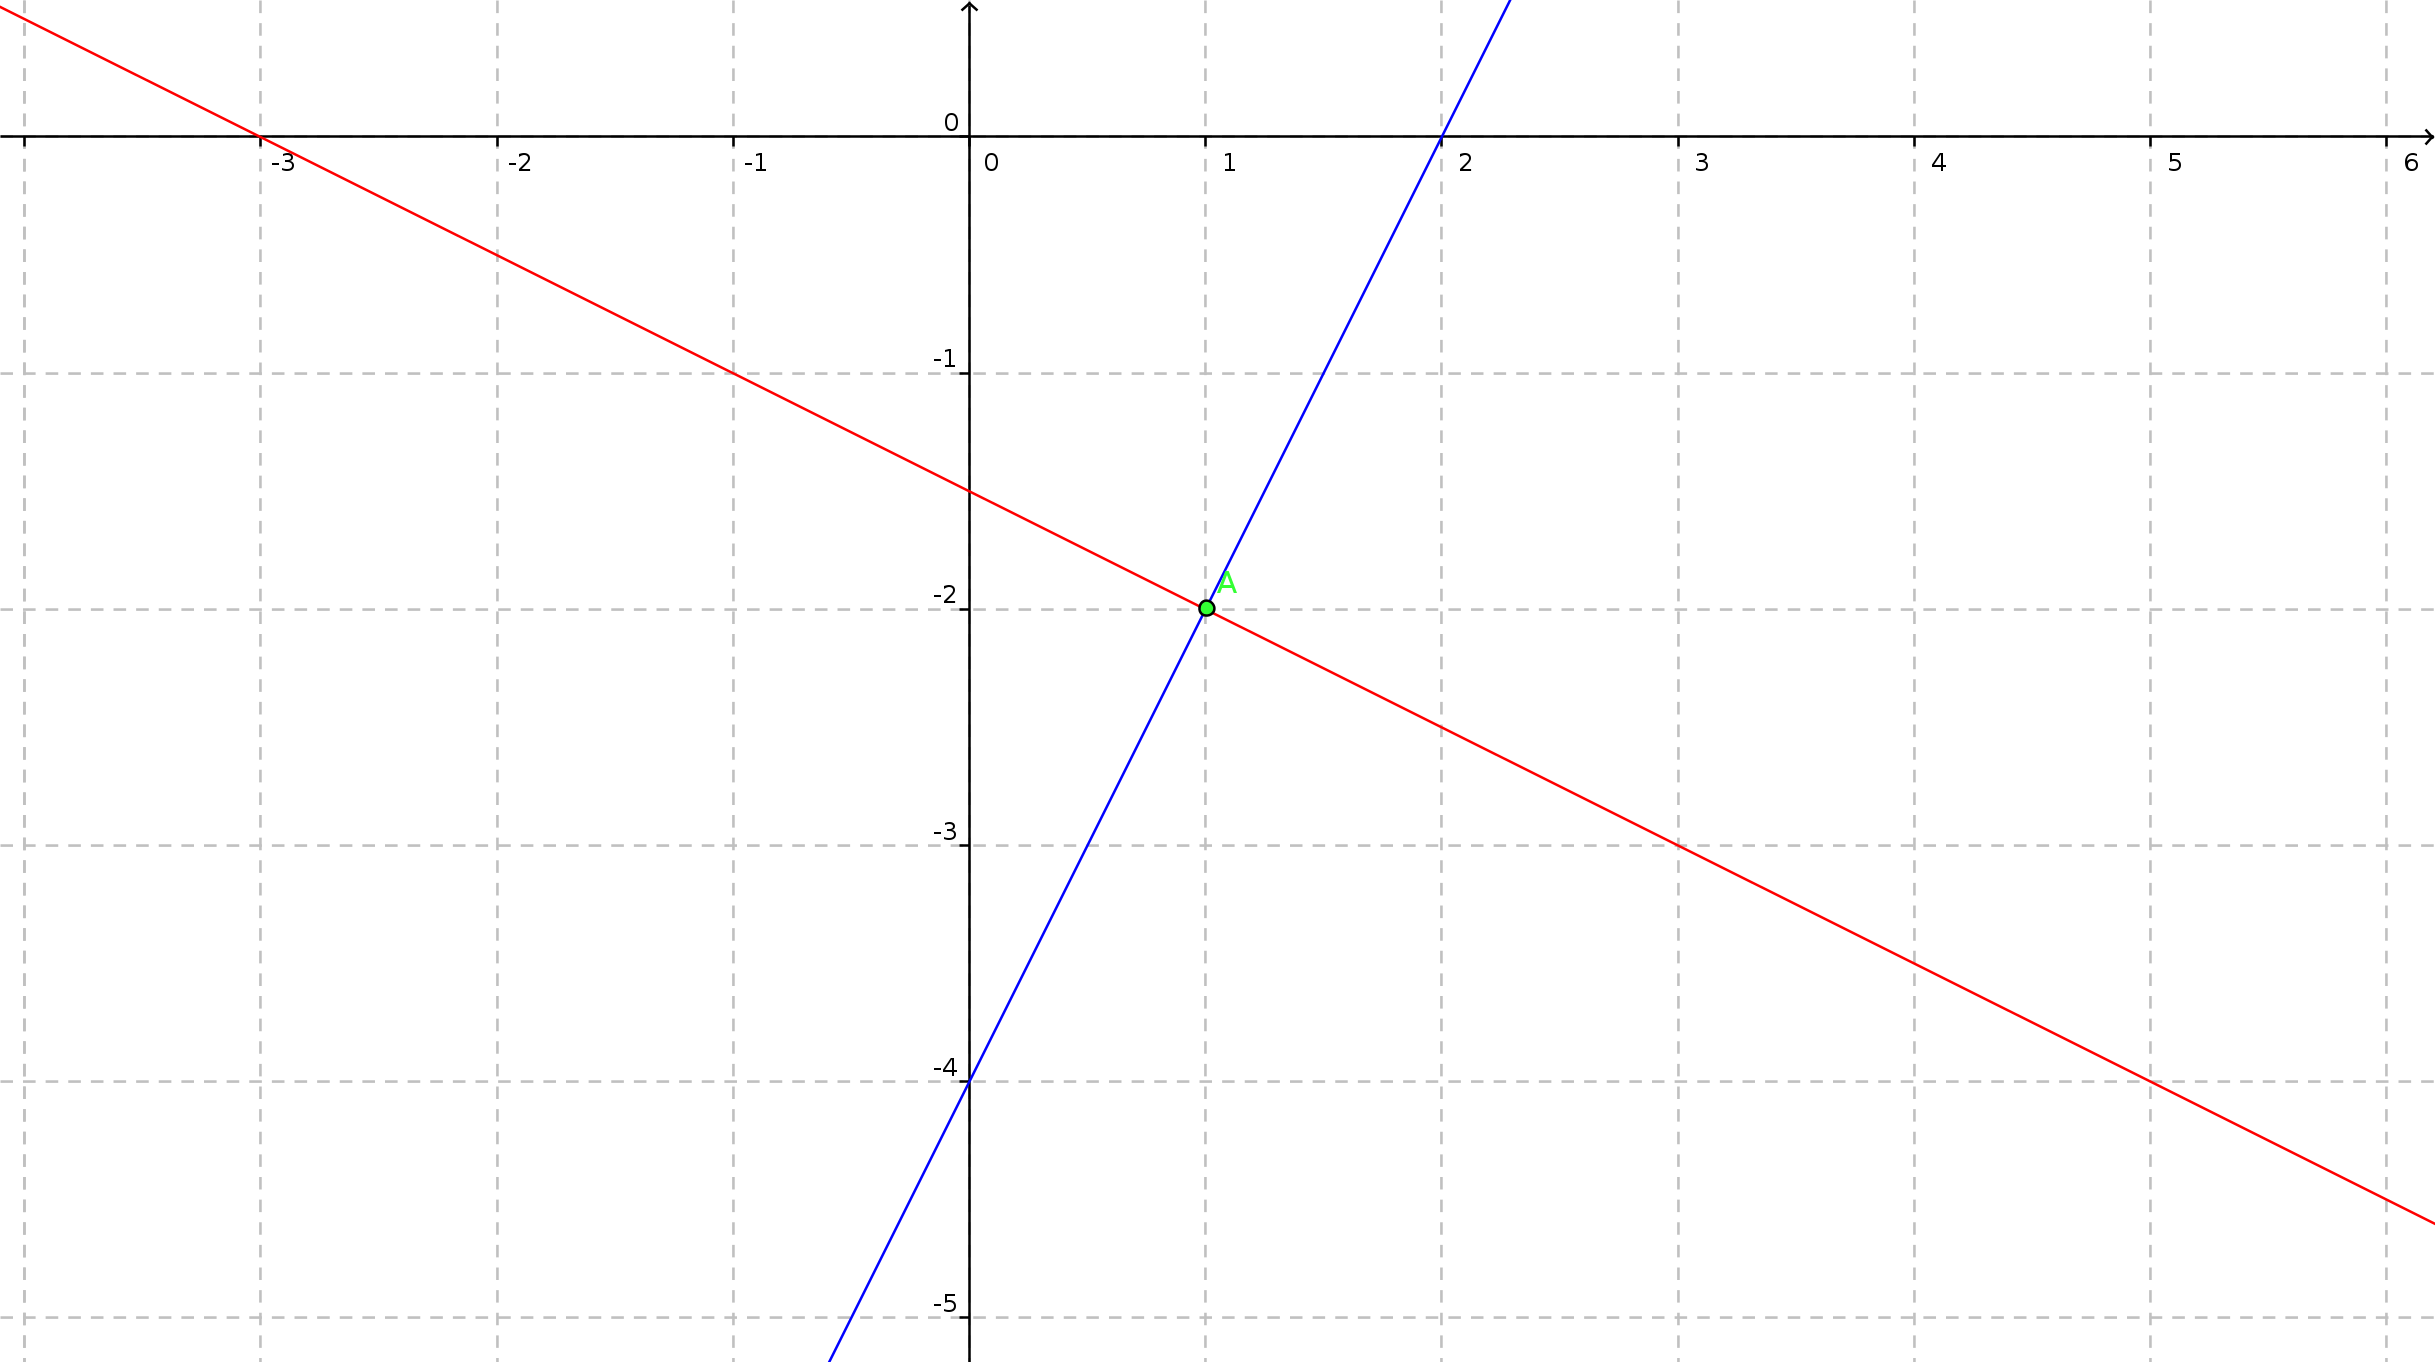
\includegraphics[height=5cm,keepaspectratio=true]{./precalculo/IM0401.png}
		% IM0401.png: 0x0 pixel, 300dpi, 0.00x0.00 cm, bb=
		\caption{$$2x-y=4\, , x+2y=-3$$}
		\label{fig:IM0401}
	\end{figure}
	


{Tipos de sistemas}
	\begin{figure}
		\centering
		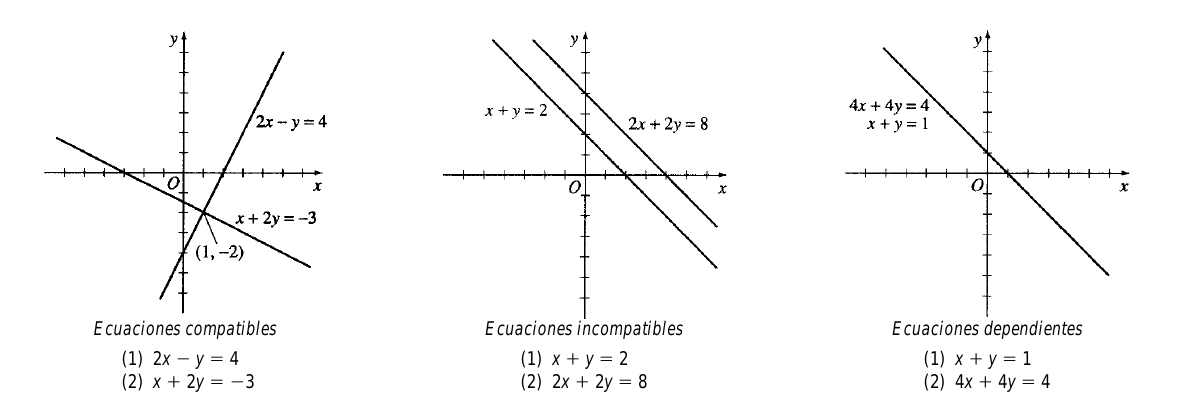
\includegraphics[width=12cm,keepaspectratio=true]{./precalculo/IM0402.png}
		% IM0402.png: 0x0 pixel, 300dpi, 0.00x0.00 cm, bb=
		\label{fig:0401}
	\end{figure}
	

